% https://tex.stackexchange.com/questions/1423/is-there-a-nice-way-to-compile-a-beamer-presentation-without-the-pauses
\documentclass[handout]{beamer}
%\documentclass[ ]{beamer}
% http://tex.stackexchange.com/questions/34265/how-to-get-beamer-math-to-look-like-article-math
% https://tex.stackexchange.com/questions/54905/how-to-modify-default-beamercolortheme
\usefonttheme[onlymath]{serif}
\pdfobjcompresslevel=0 
%\pdfminorversion=4
\include{graphix}
\include{amsmath}
%\usepackage[]{graphicx}
%\include{ulem} % strike out
% http://tex.stackexchange.com/questions/14688/put-variable-text-at-a-fixed-location-on-every-beamer-slide
\usepackage[absolute,overlay]{textpos}  
\usepackage{hyperref}
% http://tex.stackexchange.com/questions/99359/putting-animations-into-latex-beamer-presentation-use-png-gif
\usepackage{animate}
\usepackage{tikz}
% https://tex.stackexchange.com/questions/86500/includegraphics-set-image-opacity
\usepackage{transparent}
\usepackage{pgf}

% http://tex.stackexchange.com/questions/122880/continuing-example-counters-in-beamer
\setbeamertemplate{theorem}[ams style]
\setbeamertemplate{theorems}[numbered]
\newenvironment{example*}
  {\addtocounter{theorem}{-1}\example}
  {\endexample}
  
%http://tex.stackexchange.com/questions/73718/frame-numbering-in-warsaw-theme
\expandafter\def\expandafter\insertshorttitle\expandafter{%
    \insertshorttitle\hfill\insertframenumber\,/\,\inserttotalframenumber}
\expandafter\def\expandafter\insertauthor\expandafter{%
    \insertauthor\hfill\text{rev 12}}

\newcommand{\pathname}[0] {../common/}
\newcommand{\fullpath}[0] {\pathname}
\newcommand{\clr}[0]      {violet}

%\logo{\makebox[1\paperwidth]{\includegraphics[ width=1.5cm, keepaspectratio ]{../graphics/logos/HPCMP.png}}}
%\logo{\Put(-40,350){\includegraphics[ width=1.5cm, keepaspectratio ]{../graphics/logos/HPCMP.png}}}
%    {\Put(150,0){\includegraphics[ width = 4.5cm ]{../graphics/"black continuous"}}}
%\logo{\pgfputat{\pgfxy(-1,8)}{\pgfbox[center,base]{\includegraphics[width=1.6cm]{../graphics/logos/HPCMP.png}}}}  
% http://vincentwanggs.blogspot.com/2011/08/adjusting-logo-position-in-beamer.html
%\logo{\pgfputat{\pgfxy(-1,6.5)}{\pgfbox[center,base]{\includegraphics[height=0.7cm]{../graphics/logos/HPCMP.png}}}}
% http://jhshi.me/2013/12/02/place-logo-properly-in-beamer/
%\logo{\pgfputat{\pgfxy(9.45,1.5)}{\pgfbox[center,base]{\includegraphics[width=1.7cm]{../graphics/logos/HPTi.png}}}}
%\logo{\pgfputat{\pgfxy(9.45,1.5)}{\pgfbox[center,base]{\includegraphics[width=1.7cm]{../graphics/logos/HPCMP.png}}}}

% http://tex.stackexchange.com/questions/53784/overlay-images-and-block-in-beamer
%\tikzset{visib/.style={rectangle,color=blue,fill=blue!10,text=black,draw,text opacity=0.4, text width=#1,align=flush center}}
%\tikzset{invisib/.style={rectangle,color=gray,fill=gray!10,text=black,draw,text opacity=0.4, text width=#1,align=flush center}}

\input{\pathname declarations.tex}
\input{\pathname packages.tex}
%\setbeamercolor{author in head/foot}{bg=White}

% % % % % % % % % % % % % % % % % % % % % % % % % % % % % % % % % % % % % % % % % % %

\title{Orthogonality and Computation}
%\author[Topa, Embid]{\authorTopa \\ \authorEmbid }% \\ \authorTopa}
% \fontsize{20}{25}\selectfont
\author[\mg{\fontsize{5}{15}\selectfont DISTRIBUTION A. Approved for public release: distribution unlimited.}]{\authorTopa}
\institute{HPCMPO PETTT\\Engility Corp.\\ERDC DSRC\\Vicksburg MS}
%\date{29 July 2015}
\begin{document}

% http://tex.stackexchange.com/questions/237396/logo-top-right-latex-beamer-warsaw-presentation
\addtobeamertemplate{headline}{}{%
\begin{tikzpicture}[remember picture,overlay]
%\node at([shift={(.25\paperwidth,-.42)}]current page.north) {\includegraphics[ height=.5cm, width=.7cm]{../graphics/logos/HPCMP}};
%\node at([shift={(0.42\paperwidth,-0.47)}]current page.north) {\includegraphics[ height = 0.85cm]{../graphics/logos/HPTi}};
\node at([shift={(0.42\paperwidth,-0.47)}]current page.north) {\includegraphics[ height = 0.75cm ]{../graphics/logos/HPCMP}};
%\node at([shift={(-0.45\paperwidth,-0.47)}]current page.north) {\includegraphics[ height = 0.85cm ]{../graphics/logos/"logocsc"}};
\end{tikzpicture}}

%  %  %   FRAME   %   %   %
\begin{frame}
  \titlepage
%  \centering
%  Based upon presentation at
\end{frame}

%\tpage

%  %  %  %  %  %  %  %  %  %  %  %  %  %  %  %  %  %  %  %  %  %  %  %  %  %  %  %  %  %  %  %  %  %  %  %  %  %  %  %  %  %  %  %  %  %  %
\section{Problem statement}

\courtney
%\courtneyX


%  %%  %%  %%  %%  %%  %%  %%  %%  %%  %%  %%  %%  %%  %%  %%  %%  %%  %%  %%  %%  %%  %%  %%  %%  %%  %%  %%  %%  %%  %%  %%  %%  %%  %%
\subsection{Orthogonal functions}
\begin{frame}      %  %  %   FRAME   %  %  %
\frametitle{Orthogonal functions}
  %
  Popular orthogonal functions
  \begin{enumerate}
    \item sines and cosines
    \item \href{http://mathworld.wolfram.com/BesselFunction.html}{Bessel functions}
    \item \href{http://mathworld.wolfram.com/LaguerrePolynomial.html}{Laguerre polynomials}
    \item \href{http://mathworld.wolfram.com/HermitePolynomial.html}{Hermite polynomials}
    \item \href{http://mathworld.wolfram.com/ChebyshevPolynomialoftheFirstKind.html}{Chebyshev polynomials}
    \item \href{http://mathworld.wolfram.com/LegendrePolynomial.html}{Legendre polynomials}
    \item \href{http://mathworld.wolfram.com/JacobiPolynomial.html}{Jacobi polynomials}
    \item \href{http://mathworld.wolfram.com/GegenbauerPolynomial.html}{Gegenbauer polynomials}
    \item \href{http://mathworld.wolfram.com/ZernikePolynomial.html}{Zernike polynomials}
    \item \href{http://mathworld.wolfram.com/SphericalHarmonic.html}{Spherical harmonics}
  \end{enumerate}
  %
\end{frame}

\begin{frame}      %  %  %   FRAME   %  %  %
\frametitle{Orthogonal functions}
  %
  Popular orthogonal functions
  \begin{enumerate}
    \item \bl{sines and cosines}
    \item \href{http://mathworld.wolfram.com/BesselFunction.html}{Bessel functions}
    \item \href{http://mathworld.wolfram.com/LaguerrePolynomial.html}{Laguerre polynomials}
    \item \href{http://mathworld.wolfram.com/HermitePolynomial.html}{Hermite polynomials}
    \item \href{http://mathworld.wolfram.com/ChebyshevPolynomialoftheFirstKind.html}{Chebyshev polynomials}
    \item \href{http://mathworld.wolfram.com/LegendrePolynomial.html}{Legendre polynomials}
    \item \href{http://mathworld.wolfram.com/JacobiPolynomial.html}{Jacobi polynomials}
    \item \href{http://mathworld.wolfram.com/GegenbauerPolynomial.html}{Gegenbauer polynomials}
    \item \href{http://mathworld.wolfram.com/ZernikePolynomial.html}{Zernike polynomials}
    \item \href{http://mathworld.wolfram.com/SphericalHarmonic.html}{Spherical harmonics}
  \end{enumerate}
  %
    \Put(140,250){\includegraphics[ width = 1.25in ]{../graphics/extend/"trig even"}}
    \Put(230,120){\includegraphics[ width = 1.25in ]{../graphics/extend/"trig odd"}}
  %
\end{frame}

\begin{frame}      %  %  %   FRAME   %  %  %
\frametitle{Orthogonal functions}
  %
  Popular orthogonal functions
  \begin{enumerate}
    \item sines and cosines
    \item \href{http://mathworld.wolfram.com/BesselFunction.html}{\bl{Bessel functions}}
    \item \href{http://mathworld.wolfram.com/LaguerrePolynomial.html}{Laguerre polynomials}
    \item \href{http://mathworld.wolfram.com/HermitePolynomial.html}{Hermite polynomials}
    \item \href{http://mathworld.wolfram.com/ChebyshevPolynomialoftheFirstKind.html}{Chebyshev polynomials}
    \item \href{http://mathworld.wolfram.com/LegendrePolynomial.html}{Legendre polynomials}
    \item \href{http://mathworld.wolfram.com/JacobiPolynomial.html}{Jacobi polynomials}
    \item \href{http://mathworld.wolfram.com/GegenbauerPolynomial.html}{Gegenbauer polynomials}
    \item \href{http://mathworld.wolfram.com/ZernikePolynomial.html}{Zernike polynomials}
    \item \href{http://mathworld.wolfram.com/SphericalHarmonic.html}{Spherical harmonics}
  \end{enumerate}
  %
    \Put(140,250){\includegraphics[ width = 2.25in ]{../graphics/extend/"Bessels"}}
  %
\end{frame}

\begin{frame}      %  %  %   FRAME   %  %  %
\frametitle{Orthogonal functions}
  %
  Popular orthogonal functions
  \begin{enumerate}
    \item sines and cosines
    \item \href{http://mathworld.wolfram.com/BesselFunction.html}{Bessel functions}
    \item \href{http://mathworld.wolfram.com/LaguerrePolynomial.html}{\bl{Laguerre polynomials}}
    \item \href{http://mathworld.wolfram.com/HermitePolynomial.html}{Hermite polynomials}
    \item \href{http://mathworld.wolfram.com/ChebyshevPolynomialoftheFirstKind.html}{Chebyshev polynomials}
    \item \href{http://mathworld.wolfram.com/LegendrePolynomial.html}{Legendre polynomials}
    \item \href{http://mathworld.wolfram.com/JacobiPolynomial.html}{Jacobi polynomials}
    \item \href{http://mathworld.wolfram.com/GegenbauerPolynomial.html}{Gegenbauer polynomials}
    \item \href{http://mathworld.wolfram.com/ZernikePolynomial.html}{Zernike polynomials}
    \item \href{http://mathworld.wolfram.com/SphericalHarmonic.html}{Spherical harmonics}
  \end{enumerate}
  %
    \Put(140,250){\includegraphics[ width = 2.25in ]{../graphics/extend/"Laguerres"}}
  %
\end{frame}

\begin{frame}      %  %  %   FRAME   %  %  %
\frametitle{Orthogonal functions}
  %
  Popular orthogonal functions
  \begin{enumerate}
    \item sines and cosines
    \item \href{http://mathworld.wolfram.com/BesselFunction.html}{Bessel functions}
    \item \href{http://mathworld.wolfram.com/LaguerrePolynomial.html}{Laguerre polynomials}
    \item \href{http://mathworld.wolfram.com/HermitePolynomial.html}{\bl{Hermite polynomials}}
    \item \href{http://mathworld.wolfram.com/ChebyshevPolynomialoftheFirstKind.html}{Chebyshev polynomials}
    \item \href{http://mathworld.wolfram.com/LegendrePolynomial.html}{Legendre polynomials}
    \item \href{http://mathworld.wolfram.com/JacobiPolynomial.html}{Jacobi polynomials}
    \item \href{http://mathworld.wolfram.com/GegenbauerPolynomial.html}{Gegenbauer polynomials}
    \item \href{http://mathworld.wolfram.com/ZernikePolynomial.html}{Zernike polynomials}
    \item \href{http://mathworld.wolfram.com/SphericalHarmonic.html}{Spherical harmonics}
  \end{enumerate}
  %
    \Put(140,250){\includegraphics[ width = 1.25in ]{../graphics/extend/"hermite even"}}
    \Put(230,120){\includegraphics[ width = 1.25in ]{../graphics/extend/"hermite odd"}}
  %
\end{frame}

\begin{frame}      %  %  %   FRAME   %  %  %
\frametitle{Orthogonal functions}
  %
  Popular orthogonal functions
  \begin{enumerate}
    \item sines and cosines
    \item \href{http://mathworld.wolfram.com/BesselFunction.html}{Bessel functions}
    \item \href{http://mathworld.wolfram.com/LaguerrePolynomial.html}{Laguerre polynomials}
    \item \href{http://mathworld.wolfram.com/HermitePolynomial.html}{Hermite polynomials}
    \item \href{http://mathworld.wolfram.com/ChebyshevPolynomialoftheFirstKind.html}{\bl{Chebyshev polynomials}}
    \item \href{http://mathworld.wolfram.com/LegendrePolynomial.html}{Legendre polynomials}
    \item \href{http://mathworld.wolfram.com/JacobiPolynomial.html}{Jacobi polynomials}
    \item \href{http://mathworld.wolfram.com/GegenbauerPolynomial.html}{Gegenbauer polynomials}
    \item \href{http://mathworld.wolfram.com/ZernikePolynomial.html}{Zernike polynomials}
    \item \href{http://mathworld.wolfram.com/SphericalHarmonic.html}{Spherical harmonics}
  \end{enumerate}
  %
    \Put(140,250){\includegraphics[ width = 1.25in ]{../graphics/extend/"Chebyshev even"}}
    \Put(230,120){\includegraphics[ width = 1.25in ]{../graphics/extend/"Chebyshev odd"}}
  %
\end{frame}

\begin{frame}      %  %  %   FRAME   %  %  %
\frametitle{Orthogonal functions}
  %
  Popular orthogonal functions
  \begin{enumerate}
    \item sines and cosines
    \item \href{http://mathworld.wolfram.com/BesselFunction.html}{Bessel functions}
    \item \href{http://mathworld.wolfram.com/LaguerrePolynomial.html}{Laguerre polynomials}
    \item \href{http://mathworld.wolfram.com/HermitePolynomial.html}{Hermite polynomials}
    \item \href{http://mathworld.wolfram.com/ChebyshevPolynomialoftheFirstKind.html}{Chebyshev polynomials}
    \item \href{http://mathworld.wolfram.com/LegendrePolynomial.html}{\bl{Legendre polynomials}}
    \item \href{http://mathworld.wolfram.com/JacobiPolynomial.html}{\bl{Jacobi polynomials}}
    \item \href{http://mathworld.wolfram.com/GegenbauerPolynomial.html}{\bl{Gegenbauer polynomials}}
    \item \href{http://mathworld.wolfram.com/ZernikePolynomial.html}{Zernike polynomials}
    \item \href{http://mathworld.wolfram.com/SphericalHarmonic.html}{Spherical harmonics}
  \end{enumerate}
  %
    \Put(140,250){\includegraphics[ width = 1.25in ]{../graphics/extend/"Legendre even"}}
    \Put(230,120){\includegraphics[ width = 1.25in ]{../graphics/extend/"Legendre odd"}}
  %
\end{frame}

\begin{frame}      %  %  %   FRAME   %  %  %
\frametitle{Orthogonal functions}
  %
  Popular orthogonal functions
  \begin{enumerate}
    \item sines and cosines
    \item \href{http://mathworld.wolfram.com/BesselFunction.html}{Bessel functions}
    \item \href{http://mathworld.wolfram.com/LaguerrePolynomial.html}{Laguerre polynomials}
    \item \href{http://mathworld.wolfram.com/HermitePolynomial.html}{Hermite polynomials}
    \item \href{http://mathworld.wolfram.com/ChebyshevPolynomialoftheFirstKind.html}{Chebyshev polynomials}
    \item \href{http://mathworld.wolfram.com/LegendrePolynomial.html}{Legendre polynomials}
    \item \href{http://mathworld.wolfram.com/JacobiPolynomial.html}{Jacobi polynomials}
    \item \href{http://mathworld.wolfram.com/GegenbauerPolynomial.html}{Gegenbauer polynomials}
    \item \href{http://mathworld.wolfram.com/ZernikePolynomial.html}{\bl{Zernike polynomials}}
    \item \href{http://mathworld.wolfram.com/SphericalHarmonic.html}{Spherical harmonics}
  \end{enumerate}
  %
    \Put(160,200){\includegraphics[ width = 2.25in ]{../graphics/extend/"half pyramid white"}}
  %
\end{frame}

\begin{frame}      %  %  %   FRAME   %  %  %
\frametitle{Orthogonal functions}
  %
  Popular orthogonal functions
  \begin{enumerate}
    \item sines and cosines
    \item \href{http://mathworld.wolfram.com/BesselFunction.html}{Bessel functions}
    \item \href{http://mathworld.wolfram.com/LaguerrePolynomial.html}{Laguerre polynomials}
    \item \href{http://mathworld.wolfram.com/HermitePolynomial.html}{Hermite polynomials}
    \item \href{http://mathworld.wolfram.com/ChebyshevPolynomialoftheFirstKind.html}{Chebyshev polynomials}
    \item \href{http://mathworld.wolfram.com/LegendrePolynomial.html}{Legendre polynomials}
    \item \href{http://mathworld.wolfram.com/JacobiPolynomial.html}{Jacobi polynomials}
    \item \href{http://mathworld.wolfram.com/GegenbauerPolynomial.html}{Gegenbauer polynomials}
    \item \href{http://mathworld.wolfram.com/ZernikePolynomial.html}{Zernike polynomials}
    \item \href{http://mathworld.wolfram.com/SphericalHarmonic.html}{\bl{Spherical harmonics}}
  \end{enumerate}
  %
    \Put(140,200){\includegraphics[ width = 4.25in ]{../graphics/extend/"sh 04"}}
  %
\end{frame}

\begin{frame}      %  %  %   FRAME   %  %  %
\frametitle{Orthogonal functions}
  %
  Popular functions orthogonal \bl{in computation}
  \begin{enumerate}
    \item \bl{sines and cosines}
    \mg{
    \item \href{http://mathworld.wolfram.com/BesselFunction.html}{Bessel functions}
    \item \href{http://mathworld.wolfram.com/LaguerrePolynomial.html}{Laguerre polynomials}
    \item \href{http://mathworld.wolfram.com/HermitePolynomial.html}{Hermite polynomials}
    \item \href{http://mathworld.wolfram.com/ChebyshevPolynomialoftheFirstKind.html}{Chebyshev polynomials}
    \item \href{http://mathworld.wolfram.com/LegendrePolynomial.html}{Legendre polynomials}
    \item \href{http://mathworld.wolfram.com/JacobiPolynomial.html}{Jacobi polynomials}
    \item \href{http://mathworld.wolfram.com/GegenbauerPolynomial.html}{Gegenbauer polynomials}
    \item \href{http://mathworld.wolfram.com/ZernikePolynomial.html}{Zernike polynomials}
    \item \href{http://mathworld.wolfram.com/SphericalHarmonic.html}{Spherical harmonics}
    }
  \end{enumerate}
  %
\end{frame}

\begin{frame}      %  %  %   FRAME   %  %  %
\frametitle{Critical observation}
%
%\begin{textblock*}{2cm}(1cm,-7.5cm)
%  \rule{2cm}{1cm} \includegraphics[height=0.7cm]{../graphics/logos/HPCMP.png}
%\end{textblock*}  
%
  {\huge{The \rd{only} functions orthogonal in the \\
  \bl{continuum} and in \bl{discrete space}:
  $$\sin nx, \quad \cos nx$$
  } }
  %
  %
  \onedot
\end{frame}


%  %%  %%  %%  %%  %%  %%  %%  %%  %%  %%  %%  %%  %%  %%  %%  %%  %%  %%  %%  %%  %%  %%  %%  %%  %%  %%  %%  %%  %%  %%  %%  %%  %%  %%
\subsection{Summation}
\begin{frame}      %  %  %   FRAME   %  %  %
\frametitle{Rudiments}
  %
{\huge
{
  Orthogonality depends upon
  \begin{enumerate}
    \item domain
    \item topology \pause (\bl{\href{http://mathworld.wolfram.com/Continuous.html}{continuous}} or \bl{\href{http://mathworld.wolfram.com/DiscreteTopology.html}{discrete}})
  \end{enumerate}
}}
  %
\end{frame}

%%
\begin{frame}
\frametitle{Snapshot}
%
  \begin{table}[htdp]
  %\caption{}
    \begin{center}
      \begin{tabular}{ccc}
        %
        $\ L^{2}$ && $\ l^{2}$ \\
        %
        \includegraphics[ width = 1.25 in ]{../graphics/continuum.pdf} & \quad &
        %
        \includegraphics[ width = 1.25 in ]{../graphics/discrete.pdf}
        %
        %
      \end{tabular}
    \end{center}
  \label{tab:lines}
\end{table}%
%
%\pause
%
{\huge
{
  $$\href{http://mathworld.wolfram.com/Lp-Space.html}{L^{2}} \text{ is not } l^{2} $$
}}
%
%\pause
%
\begin{center}
{\Large
{
That's why they have different symbols
}}
\end{center}
\twodots
%
\end{frame}

%  %  %  %  %  %  %  %  %  %  %  %  %  %  %  %  %  %  %  %  %  %  %  %  %  %  %  %  %  %  %  %  %  %  %  %  %  %  %  %  %  %  %  %  %  %  %
% https://tex.stackexchange.com/questions/68266/light-gray-color-in-beamer
\colorlet{shadecolor}{gray!80}

%  %  %  %  %  %  %  %  %  %  %  %  %  %  %  %  %  %  %  %  %  %  %  %  %  %  %  %  %  %  %  %  %  %  %  %  %  %  %  %  %  %  %  %  %  %  %
\section{Paean to orthogonality}


%  %%  %%  %%  %%  %%  %%  %%  %%  %%  %%  %%  %%  %%  %%  %%  %%  %%  %%  %%  %%  %%  %%  %%  %%  %%  %%  %%  %%  %%  %%  %%  %%  %%  %%
\subsection{Linear Systems}
 
\begin{frame}      %  %  %   FRAME   %  %  %
\frametitle{Prototype linear equation}
  %
  {\Huge{$$\mathbf{A}x=b$$}}
  %
  $$x_{1} \bl{\mat{c}{a_{11}\\\vdots\\a_{m1}}}+\dots+
    x_{n} \bl{\mat{c}{a_{1n}\\\vdots\\a_{mn}}} = \mat{c}{b_{1}\\\vdots\\b_{m}}$$
  %
\end{frame}

\begin{frame}
  \frametitle{Condition Number}  % - - - - F R A M E
  %
  %\animategraphics[ autoplay,loop, width = 4.5in ]{4}{../graphics/animation/"panels "}{10}{51}
  \animategraphics[ autoplay, loop, width = 4.5in ]{4}{../graphics/animation/"p_"}{1}{57}
  %
\end{frame}


\begin{frame}      %  %  %   FRAME   %  %  %
\frametitle{Column vectors of $\mathbf{A}$}
  %
  \begin{table}[htdp]
    %\caption{default}
    \begin{center}
      \begin{tabular}{cccc}
        %
        \includegraphics[width = 2.1cm ]{../graphics/"cases a"} & 
        %
        \includegraphics[width = 2.1cm ]{../graphics/"cases b"} & 
        %
        \includegraphics[width = 2.1cm ]{../graphics/"cases c"} & 
        %\pause
        %
        \includegraphics[width = 2.1cm ]{../graphics/"cases d"} \\ 
        %
        linearly & linearly  & orthogonal & diagonal \\
        %
        dependent & independent
        %
      \end{tabular}
    \end{center}
    %\label{default}
  \end{table}%
  %
%  \pause
%  %
%  \begin{center}
%    BAD \qquad \qquad \qquad $\longrightarrow$ \qquad \qquad \qquad GOOD
%  \end{center}
  %
\end{frame}

%\begin{frame}      %  %  %   FRAME   %  %  %
%\frametitle{Column vectors of $\mathbf{A}$: solution tools}
%  %
%  \begin{table}[htdp]
%    %\caption{default}
%    \begin{center}
%      \begin{tabular}{cccc}
%        %
%        \multicolumn{2}{c}{SVD, QR} & GE, LU &
%        %
%        $x_{r} = b_{r} / a_{rr}$ \\
%        %
%        \includegraphics[width = 2.1cm ]{../graphics/"cases a"} & 
%        %
%        \includegraphics[width = 2.1cm ]{../graphics/"cases b"} & 
%        %
%        \includegraphics[width = 2.1cm ]{../graphics/"cases c"} & 
%        %
%        \includegraphics[width = 2.1cm ]{../graphics/"cases d"} \\ 
%        %
%        linearly & linearly  & orthogonal & diagonal \\
%        %
%        dependent & independent
%        %
%      \end{tabular}
%    \end{center}
%    %\label{default}
%  \end{table}%
%\end{frame}

\begin{frame}      %  %  %   FRAME   %  %  %
\frametitle{Column vectors of $\mathbf{A}$: clicks}
  %
  \begin{table}[htdp]
    %\caption{default}
    \begin{center}
      \begin{tabular}{ccc|c}
        %
        %SVD & QR, PLU & GE, LU &
        &&&
        %
        $x_{r} = b_{r} / a_{rr}$ \\
        %
        \includegraphics[width = 2.1cm ]{../graphics/"cases a"} & 
        %
        \includegraphics[width = 2.1cm ]{../graphics/"cases b"} & 
        %
        \includegraphics[width = 2.1cm ]{../graphics/"cases c"} & 
        %
        \includegraphics[width = 2.1cm ]{../graphics/"cases d"} \\ 
        %
        linearly & linearly  & orthogonal & diagonal \\
        %
        dependent & independent
        %
      \end{tabular}
    \end{center}
    %\label{default}
  \end{table}%
  %
%  \pause
%  %
%  \begin{center}
%    BAD \qquad \qquad \qquad $\longrightarrow$ \qquad \qquad \qquad GOOD
%  \end{center}
  %
\end{frame}	
% https://tex.stackexchange.com/questions/8043/change-the-background-color-of-a-frame-in-beamer
%{\setbeamercolor{background canvas}{bg = shadecolor}

{
{\setbeamercolor{background canvas}{bg=gray!90}
\begin{frame}      %  %  %   FRAME   %  %  %
\frametitle{Column vectors of $\mathbf{A}$: $L^{2}$}
  %
  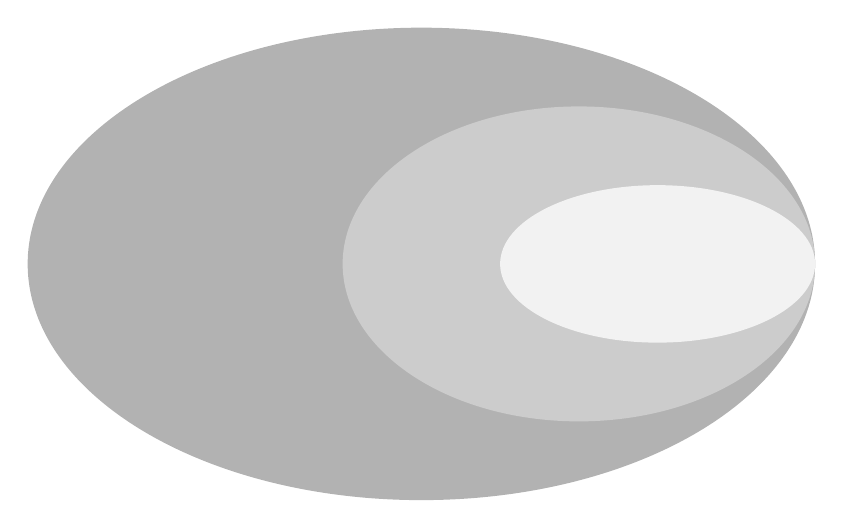
\begin{tikzpicture}
    \fill[gray!60] ellipse (5cm and 3cm);
    \fill[gray!40](2cm,0cm) ellipse (3cm and 2cm);
    \fill[gray!10](3cm,0cm) ellipse (2cm and 1cm);
  \end{tikzpicture}
  %
    \begin{textblock*}{5cm}(3.5cm,3.25cm)%
     Linearly Independent
  \end{textblock*}
  %
  \begin{textblock*}{5cm}(6.5cm,4.15cm)%
     Orthogonal
  \end{textblock*}
  %
  \begin{textblock*}{5cm}(7.95cm,4.95cm)%
     Diagonal
  \end{textblock*}
%      {\scriptsize{
      {\tiny{
      %%
      \begin{textblock*}{5cm}(9.1cm, 5.4cm)%
         \bl{trigonometric}
      \end{textblock*}
      %%
      \begin{textblock*}{5cm}(7.1cm, 5.40cm)%
         \bl{Zernike}
      \end{textblock*}
      %%
      \begin{textblock*}{5cm}(7.5cm, 5.70cm)%
         \bl{Legendre}
      \end{textblock*}
      %%
      \begin{textblock*}{5cm}(7.9cm, 6.00cm)%
         \bl{Hermite}
      \end{textblock*}
      %%
      \begin{textblock*}{5cm}(8.55cm, 6.30cm)%
         \bl{Bessel}
      \end{textblock*}
      %%
      \begin{textblock*}{5cm}(8.3cm, 5.45cm)%
         \bl{Jacobi}
      \end{textblock*}
      %%
      \begin{textblock*}{5cm}(8.6cm, 5.85cm)%
         \bl{Gegenbauer}
      \end{textblock*}
      %%
      \begin{textblock*}{5cm}(9.4cm, 6.1cm)%
         \bl{Chebyshev}
      \end{textblock*}
      %%
      \begin{textblock*}{5cm}(8.9cm, 5.65cm)%
         \bl{Spherical harmonics}
      \end{textblock*}
      %%
      \begin{textblock*}{5cm}(9.5cm, 5.0cm)%
         \bl{Laguerre}
      \end{textblock*}
      %%
      %%
      }}
      %%
\end{frame}
}}

{
{\setbeamercolor{background canvas}{bg=gray!90}
\begin{frame}      %  %  %   FRAME   %  %  %
\frametitle{Column vectors of $\mathbf{A}$: $l^{2}$}
  %
  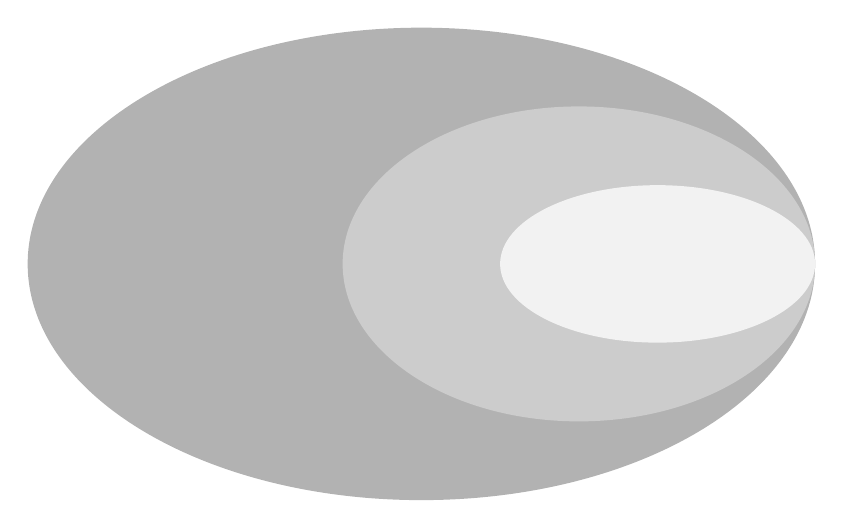
\begin{tikzpicture}
    \fill[gray!60] ellipse (5cm and 3cm);
    \fill[gray!40](2cm,0cm) ellipse (3cm and 2cm);
    \fill[gray!10](3cm,0cm) ellipse (2cm and 1cm);
  \end{tikzpicture}
  %
    %
  \begin{textblock*}{5cm}(3.5cm,3.25cm)%
     Linearly Independent
  \end{textblock*}
  %
  \begin{textblock*}{5cm}(6.5cm,4.15cm)%
     Orthogonal
  \end{textblock*}
  %
  \begin{textblock*}{5cm}(7.95cm,4.95cm)%
     Diagonal
  \end{textblock*}
%      {\scriptsize{
%      {\tiny{
      {\footnotesize{
      %%
      \begin{textblock*}{5cm}(8.5cm, 5.5cm)%
         \bl{trigonometric}
      \end{textblock*}
      %%
      \begin{textblock*}{5cm}(3.3cm, 5.40cm)%
         \bl{Gegenbauer}
      \end{textblock*}
      %%
      \begin{textblock*}{5cm}(3.7cm, 5.70cm)%
         \bl{Legendre}
      \end{textblock*}
      %%
      \begin{textblock*}{5cm}(3.9cm, 6.00cm)%
         \bl{Hermite}
      \end{textblock*}
      %%
      \begin{textblock*}{5cm}(4.2cm, 6.30cm)%
         \bl{Bessel}
      \end{textblock*}
      %%
      \begin{textblock*}{5cm}(4.1cm, 5.1cm)%
         \bl{Jacobi}
      \end{textblock*}
      %%
      \begin{textblock*}{5cm}(4.1cm, 4.8cm)%
         \bl{Zernike}
      \end{textblock*}
      %%
      \begin{textblock*}{5cm}(3.8cm, 6.60cm)%
         \bl{Chebyshev}
      \end{textblock*}
      %%
      \begin{textblock*}{5cm}(3.3cm, 7.2cm)%
         \bl{Spherical harmonics}
      \end{textblock*}
      %%
      \begin{textblock*}{5cm}(4.35cm, 6.9cm)%
         \bl{Laguerre}
      \end{textblock*}
      %%
      %%
      }}
      %%
      \onedot
\end{frame}
}}

%  %%  %%  %%  %%  %%  %%  %%  %%  %%  %%  %%  %%  %%  %%  %%  %%  %%  %%  %%  %%  %%  %%  %%  %%  %%  %%  %%  %%  %%  %%  %%  %%  %%  %%
\subsection{General case}

\begin{frame}      %  %  %   FRAME   %  %  %
\frametitle{General System}
	$$
	\mathbf{A} x = b
	$$\\[10pt]
  $$
  \mat{cc}{ a_{11} & \rd{a_{12}} \\ \rd{a_{21}} & a_{22} }
  \mat{c}{x_{1} \\ x_{2}} =
  \mat{c}{b_{1} \\ b_{2}}
  $$
  %
  %\pause
  \begin{center}
  $\Downarrow$
  \end{center}
  %
  $$
  \mat{c}{x_{1} \\ x_{2}} = 
  {\rd{\mat{cc}{ a_{11} & a_{12} \\ a_{21} & a_{22} }^{-1}}}
  \mat{c}{b_{1} \\ b_{2}}
  $$
  %
  \onedot
\end{frame}


%  %%  %%  %%  %%  %%  %%  %%  %%  %%  %%  %%  %%  %%  %%  %%  %%  %%  %%  %%  %%  %%  %%  %%  %%  %%  %%  %%  %%  %%  %%  %%  %%  %%  %%
\subsection{Diagonal matrices}
\begin{frame}      %  %  %   FRAME   %  %  %
\frametitle{Diagonal System}
	$$
	\mathbf{A} x = b
	$$\\[10pt]
  $$
  \mat{cc}{ \alpha_{1} & \bzero \\ \bzero & \alpha_{2} }
  \mat{c}{x_{1} \\ x_{2}} =
  \mat{c}{b_{1} \\ b_{2}}
  $$
  %
  %\pause
  \begin{center}
  $\Downarrow$
  \end{center}
  %
  $$
  \mat{c}{x_{1} \\ x_{2}} = 
  {\color{blue}{\mat{cc}{1/\alpha_{1} & 0 \\ 0 & 1/\alpha_{2} }}}
  \mat{c}{b_{1} \\ b_{2}}
  $$
  %
\end{frame}

\begin{frame}      %  %  %   FRAME   %  %  %
\frametitle{Decoupling Principle}
  %
  \bl{Diagonal} Systems are \bl{Decoupled} \\
   \Put(220,-250) {\href{http://www.ams.org/bookstore-getitem/item=MBK-50}{\includegraphics[ height = 5cm ]{../graphics/"sadun"}}}
  %\Put(220,-250) {\href{http://www.ams.org/bookstore-getitem/item=MBK-50}{\includegraphics[ height = 5cm ]{../graphics/"caution"}}}
  %
    \pause
  %
\begin{itemize}
  \item  difference equations
  \item  Markov chains
  \item  coupled oscillators
  \item  Fourier series
  \item  wave equation
  \item  Schrodinger equation
\end{itemize}
  %
  %
  %
  \twodots
\end{frame}

%  %  %  %  %  %  %  %  %  %  %  %  %  %  %  %  %  %  %  %  %  %  %  %  %  %  %  %  %  %  %  %  %  %  %  %  %  %  %  %  %  %  %  %  %  %  %
\section{Lebesgue spaces}


%  %%  %%  %%  %%  %%  %%  %%  %%  %%  %%  %%  %%  %%  %%  %%  %%  %%  %%  %%  %%  %%  %%  %%  %%  %%  %%  %%  %%  %%  %%  %%  %%  %%  %%
\subsection{Intuition}

\begin{frame}      %  %  %   FRAME   %  %  %
\frametitle{$L^{2}$: Legendre Basis}
  %
  $$F(x) \approx \sum_{k=0}^{d} \bl{a_{k}}P_{k}(x)$$\\[7pt]	
  %
  \raisebox{-0.5\height}{ \includegraphics[ width = 1.75cm ]{../graphics/approximation/"in smooth"} } = 
  $a_{0}$ \!\!\! \raisebox{-0.5\height}{ \includegraphics[ width = 1.75cm ]{../graphics/approximation/"leg 00"} } +
  $a_{1}$ \!\!\! \raisebox{-0.5\height}{ \includegraphics[ width = 1.75cm ]{../graphics/approximation/"leg 01"} } +
  $a_{2}$ \!\!\! \raisebox{-0.5\height}{ \includegraphics[ width = 1.75cm ]{../graphics/approximation/"leg 02"} } \\[7pt]
  \qquad \qquad \quad \ +
  %
  $a_{3}$ \!\!\! \raisebox{-0.5\height}{ \includegraphics[ width = 1.75cm ]{../graphics/approximation/"leg 03"} } +
  $a_{4}$ \!\!\! \raisebox{-0.5\height}{ \includegraphics[ width = 1.75cm ]{../graphics/approximation/"leg 04"} } +
  $a_{5}$ \!\!\! \raisebox{-0.5\height}{ \includegraphics[ width = 1.75cm ]{../graphics/approximation/"leg 05"} } 
  %
\end{frame}


\begin{frame}      %  %  %   FRAME   %  %  %
\frametitle{$l^{2}$: Legendre Basis}
  %
  $$f(x) \approx \sum_{k=0}^{d} \bl{b_{k}}P_{k}(x)$$\\[7pt]	
  %
  \raisebox{-0.5\height}{ \includegraphics[ width = 1.75cm ]{../graphics/approximation/"in smooth discrete"} } = 
  $b_{0}$ \!\!\!\raisebox{-0.5\height}{ \includegraphics[ width = 1.75cm ]{../graphics/approximation/"discrete leg 00"} } +
  $b_{1}$ \!\!\!\raisebox{-0.5\height}{ \includegraphics[ width = 1.75cm ]{../graphics/approximation/"discrete leg 01"} } +
  $b_{2}$ \!\!\!\raisebox{-0.5\height}{ \includegraphics[ width = 1.75cm ]{../graphics/approximation/"discrete leg 02"} } \\[7pt]
  \qquad \qquad \quad \ +
  %
  $b_{3}$ \!\!\!\raisebox{-0.5\height}{ \includegraphics[ width = 1.75cm ]{../graphics/approximation/"discrete leg 03"} } +
  $b_{4}$ \!\!\!\raisebox{-0.5\height}{ \includegraphics[ width = 1.75cm ]{../graphics/approximation/"discrete leg 04"} } +
  $b_{5}$ \!\!\!\raisebox{-0.5\height}{ \includegraphics[ width = 1.75cm ]{../graphics/approximation/"discrete leg 05"} } 
  %
\end{frame}

\begin{frame}
\frametitle{Finding the Amplitudes}
  \Large{Finding amplitudes = Solving linear systems}
  \onedot
\end{frame} 


%  %%  %%  %%  %%  %%  %%  %%  %%  %%  %%  %%  %%  %%  %%  %%  %%  %%  %%  %%  %%  %%  %%  %%  %%  %%  %%  %%  %%  %%  %%  %%  %%  %%  %%
\subsection{Formalism}
\begin{frame}
  \frametitle{Formalities}  % - - - - F R A M E
  %
  \centering
  \includegraphics[ width = 3.75in ]{../graphics/approximation/paper}
  %
  \Put(-20,350){\includegraphics[ height = 0.85cm ]{../graphics/logos/"logocsc"}}
  %
\end{frame}


\begin{frame}      %  %  %   FRAME   %  %  %
\frametitle{Riesz-Fischer}
  %
 % http://tex.stackexchange.com/questions/136589/colour-themes-in-beamer-not-working-for-lemma-theorem-definition-environments
 \setbeamercolor{structure}{fg=darkred}
 \setbeamercolor{block body}{bg=gray!10!white}
   \begin{theorem}[Riesz--Fischer]
Let $\lst{\phi_{n}}$ be an \bl{orthonormal} sequence of functions on $\Omega$ and suppose $\sum \abs{a_{n}}^{2}$ converges. Denote the partial sum as
  % % % EQUATION
  \begin{equation*}
    s_{d} = a_{0}\phi_{0} + a_{1}\phi_{1} + \cdots + a_{d}\phi_{d} .
  \end{equation*}
  % % %
There exists a function $F\in\spaceL$ such that $\lst{s_{d}}$ \bl{converges} to $F$ in $\spaceL$, and such that
  % % % EQUATION
  \begin{equation*}
    F = \sum_{k=0}^{\infty} a_{k}\phi_{k},
  \end{equation*}
  % % %
almost everywhere.
\end{theorem}
  %
\end{frame}


\begin{frame}      %  %  %   FRAME   %  %  %
  \frametitle{Normal Equations: General Case}
  \footnotesize{
\begin{table}[htdp]
    %\caption{default}
    \begin{center}
        \begin{tabular}{ccccc}
          %
          & system & sol'n && data \\[10pt]
          %
          %
            $L^{2}$: & 
          %
            $\mat{cccc}{
            \innerx{G_{0}}{G_{0}} & \innerx{G_{0}}{G_{1}} & \cdots & \innerx{G_{0}}{G_{d}} \\
            \innerx{G_{1}}{G_{0}} & \innerx{G_{1}}{G_{1}} & \cdots & \innerx{G_{1}}{G_{d}} \\
            \vdots & \vdots & \ddots & \vdots \\
            \innerx{G_{d}}{G_{0}} & \innerx{G_{d}}{G_{1}} & \cdots & \innerx{G_{d}}{G_{d}}
            }$ &
          %
            $\pr{\mat{c}{ a_{0} \\ a_{1} \\ \vdots \\ a_{d} }}$ & = &
          %
            $\mat{c}{ \innerx{F}{G_{0}} \\ \innerx{F}{G_{1}} \\ \vdots \\ \innerx{F}{G_{d}} }$ \\[35pt]
          %%%
            $l^{2}$: &
          %
            $\mat{cccc}{
            \innerx{g_{0}}{g_{0}} & \innerx{g_{0}}{g_{1}} & \cdots & \innerx{g_{0}}{g_{d}} \\
            \innerx{g_{1}}{g_{0}} & \innerx{g_{1}}{g_{1}} & \cdots & \innerx{g_{1}}{g_{d}} \\
            \vdots & \vdots & \ddots & \vdots \\
            \innerx{g_{d}}{g_{0}} & \innerx{g_{d}}{g_{1}} & \cdots & \innerx{g_{d}}{g_{d}}
            }$ &
          %
            $\pr{\mat{c}{ b_{0} \\ b_{1} \\ \vdots \\ b_{d} }}$ & = &
          %
            $\mat{c}{ \innerx{f}{g_{0}} \\ \innerx{f}{g_{1}} \\ \vdots \\ \innerx{f}{g_{d}} }$          
          %
        \end{tabular}
    \end{center}
    %\label{default}
\end{table}%
}
\end{frame}

\begin{frame}      %  %  %   FRAME   %  %  %
  \frametitle{Expression of Orthogonality}
    %
    $$m\ne n$$
    %
\begin{table}[htdp]
    %\caption{default}
    \begin{center}
        \begin{tabular}{cccccc}
          $L^{2}$: & $\innerx{G_{m}}{G_{n}}$ & = & $\int\limits_{\Omega} G_{m}(x) G_{n}(x) dx$ & = & 0\\[30pt]
          %\pause
          %
          $l^{2}$: & $\innerx{g_{m}}{g_{n}}$ & = & $\sum\limits_{x\in\sigma} g_{m}(x) g_{n}(x) \Delta$ & = & 0
        \end{tabular}
    \end{center}
    %\label{default}
\end{table}%  
    %
    %
\end{frame}


\begin{frame}      %  %  %   FRAME   %  %  %
  \frametitle{Normal Equations: Orthogonal Basis}
  \footnotesize{
\begin{table}[htdp]
    %\caption{default}
    \begin{center}
        \begin{tabular}{ccccc}
          %
          & system & sol'n && data \\[10pt]
          %
            $L^{2}$: & 
          %
            $\mat{cccc}{
            \innerx{G_{0}}{G_{0}} & \bzero & \cdots & \bzero \\
            \bzero & \innerx{G_{1}}{G_{1}} & \cdots & \bzero \\
            \vdots & \vdots & \ddots & \vdots \\
            \bzero & \bzero & \cdots & \innerx{G_{d}}{G_{d}}
            }$ &
          %
            $\pr{\mat{c}{ a_{0} \\ a_{1} \\ \vdots \\ a_{d} }}$ & = &
          %
            $\mat{c}{ \innerx{F}{G_{0}} \\ \innerx{F}{G_{1}} \\ \vdots \\ \innerx{F}{G_{d}} }$ \\[35pt]
          %%%
            $l^{2}$: &
          %
            $\mat{cccc}{
            \innerx{g_{0}}{g_{0}} & \bzero & \cdots & \bzero \\
            \bzero & \innerx{g_{1}}{g_{1}} & \cdots & \bzero \\
            \vdots & \vdots & \ddots & \vdots \\
            \bzero & \bzero & \cdots & \innerx{g_{d}}{g_{d}}
            }$ &
          %
            $\pr{\mat{c}{ b_{0} \\ b_{1} \\ \vdots \\ b_{d} }}$ & = &
          %
            $\mat{c}{ \innerx{f}{g_{0}} \\ \innerx{f}{g_{1}} \\ \vdots \\ \innerx{f}{g_{d}} }$          
          %
        \end{tabular}
    \end{center}
    %\label{default}
\end{table}%
}
\end{frame}


\begin{frame}      %  %  %   FRAME   %  %  %
\frametitle{In a Nutshell}
  %
\begin{table}[htdp]
  %\caption{default}
  \begin{center}
    \begin{tabular}{cc}
      %
      \ $L^{2}$ & \qquad \ $l^{2}$ \\\hline
      %
      %
      &\\
      \includegraphics[ width = 3.75cm ]{../graphics/"area cont"} & \qquad
      \includegraphics[ width = 3.75cm ]{../graphics/"area disc"} \\
      %
      $ \ \innerx{G_{m}}{G_{n}} $ & \qquad \ $ \innerx{g_{m}}{g_{n}} $ \\[8pt]
      %\pause
      $ \int\limits_{\Omega} P_{m}(x) P_{n}(x) dx \ \bl{= 0} $ & \qquad
      $ \sum\limits_{x\in\sigma} P_{m}(x) P_{n}(x) \Delta \ \rd{\ne 0}$
      %
    \end{tabular}
  \end{center}
  %\label{default}
\end{table}%
\twodots
  %
\end{frame}

%  %  %  %  %  %  %  %  %  %  %  %  %  %  %  %  %  %  %  %  %  %  %  %  %  %  %  %  %  %  %  %  %  %  %  %  %  %  %  %  %  %  %  %  %  %  %
\section{Computation in $l^{2}$}
{
{\setbeamercolor{background canvas}{bg=black}
{\tc{

%  %%  %%  %%  %%  %%  %%  %%  %%  %%  %%  %%  %%  %%  %%  %%  %%  %%  %%  %%  %%  %%  %%  %%  %%  %%  %%  %%  %%  %%  %%  %%  %%  %%  %%
\subsection{Examples}
\begin{frame}      %  %  %   FRAME   %  %  %
\frametitle{Smoothness}
  %
  \begin{center}
    \includegraphics[ width = 4cm ]{../graphics/"black continuous".pdf} \qquad \qquad 
    \includegraphics[ width = 4cm ]{../graphics/"black discontinuous".pdf} 
  \end{center}
  %
  \donedot
\end{frame}

%  %%  %%  %%  %%  %%  %%  %%  %%  %%  %%  %%  %%  %%  %%  %%  %%  %%  %%  %%  %%  %%  %%  %%  %%  %%  %%  %%  %%  %%  %%  %%  %%  %%  %%
\subsection{Continuous function}

\begin{frame}      %  %  %   FRAME   %  %  %
\frametitle{Monomials and Legendre Polynomials}
  %
\footnotesize{
\begin{table}[htdp]
  %\caption{default}
  \begin{center}
    \begin{tabular}{rcl}
      %
      $k$ & $M_{k}(x)$ & $P_{k}(x)$ \\\hline
      %
       0 & $1$ & $1$ \\
       1 & $x$ & $x$ \\
       2 & $x^2$ & $\frac{1}{2} \left(3 x^2-1\right)$ \\[3pt]
       3 & $x^3$ & $\frac{1}{2} \left(5 x^3-3 x\right)$ \\[3pt]
       4 & $x^4$ & $\frac{1}{8} \left(35 x^4-30 x^2+3\right)$ \\[3pt]
       5 & $x^5$ & $\frac{1}{8} \left(63 x^5-70 x^3+15 x\right)$ \\[3pt]
       6 & $x^6$ & $\frac{1}{16} \left(231 x^6-315 x^4+105 x^2-5\right)$ \\[3pt]
       7 & $x^7$ & $\frac{1}{16} \left(429 x^7-693 x^5+315 x^3-35 x\right)$ \\[3pt]
       8 & $x^8$ & $\frac{1}{128} \left(6435 x^8-12012 x^6+6930 x^4-1260 x^2+35\right)$ \\[3pt]
       9 & $x^9$ & $\frac{1}{128} \left(12155 x^9-25740 x^7+18018 x^5-4620 x^3+315 x\right)$ \\[3pt]
       10 & $x^{10}$ & $\frac{1}{256} \left(46189 x^{10}-109395 x^8+90090 x^6-30030 x^4+3465 x^2-63\right)$
      %
      %
    \end{tabular}
  \end{center}
  \label{default}
\end{table}%
       }
  %
\end{frame}


\begin{frame}      %  %  %   FRAME   %  %  %
  \frametitle{Comparing methods}
  %
\begin{table}[htdp]
    %\caption{Comparing methods}
    \begin{center}
        \begin{tabular}{lcc}
          %
           & faux & linear \\
           & orthogonality & independence \\\hline
          %
          \gr{mesh points} & \rd{$10^{9}$} & 9 \\
          %
          \gr{error} & \rd{$10^{-9}$} & 0
          %
          %
        \end{tabular}
    \end{center}
    %\label{default}
\end{table}%
  %
  %
  \dtwodots
\end{frame}


%  %%  %%  %%  %%  %%  %%  %%  %%  %%  %%  %%  %%  %%  %%  %%  %%  %%  %%  %%  %%  %%  %%  %%  %%  %%  %%  %%  %%  %%  %%  %%  %%  %%  %%
\subsection{Discontinuous Function}

\begin{frame}      %  %  %   FRAME   %  %  %
  \frametitle{Monomials: Degree of fit = 50}
  \begin{table}[htdp]
    %\caption{default}
     \begin{center}
        \begin{tabular}{cc}
          %
          amplitudes & approximation \\[10pt]
          %
          \includegraphics[ width = 4cm ]{../graphics/"black sign amp 050"} &
          \includegraphics[ width = 4cm ]{../graphics/"black sign fit 050"}
          %
          %
        \end{tabular}
     \end{center}
    %\label{default}
  \end{table}% 
\end{frame}

\begin{frame}      %  %  %   FRAME   %  %  %
  \frametitle{Monomials: Degree of fit = 100}
  \begin{table}[htdp]
    %\caption{default}
     \begin{center}
        \begin{tabular}{cc}
          %
          amplitudes & approximation \\[10pt]
          %
          \includegraphics[ width = 4cm ]{../graphics/"black sign amp 100"} &
          \includegraphics[ width = 4cm ]{../graphics/"black sign fit 100"}
          %
          %
        \end{tabular}
     \end{center}
    %\label{default}
  \end{table}% 
\end{frame}

\begin{frame}      %  %  %   FRAME   %  %  %
  \frametitle{Monomials: Degree of fit = 200}
  \begin{table}[htdp]
    %\caption{default}
     \begin{center}
        \begin{tabular}{cc}
          %
          amplitudes & approximation \\[10pt]
          %
          \includegraphics[ width = 4cm ]{../graphics/"black sign amp 200"} &
          \includegraphics[ width = 4cm ]{../graphics/"black sign fit 200"}
          %
          %
        \end{tabular}
     \end{center}
    %\label{default}
  \end{table}% 
  \donedot
\end{frame}

\begin{frame}      %  %  %   FRAME   %  %  %
  \frametitle{Legendre Polynomials: Degree of fit = 50}
  \begin{table}[htdp]
    %\caption{default}
     \begin{center}
        \begin{tabular}{cc}
          %
          amplitudes & approximation \\[10pt]
          %
          \includegraphics[ width = 4cm ]{../graphics/"black sign leg 050"} &
          \includegraphics[ width = 4cm ]{../graphics/"black sign fit 050"}
          %
          %
        \end{tabular}
     \end{center}
    %\label{default}
  \end{table}% 
\end{frame}

\begin{frame}      %  %  %   FRAME   %  %  %
  \frametitle{Legendre Polynomials: Degree of fit = 100}
  \begin{table}[htdp]
    %\caption{default}
     \begin{center}
        \begin{tabular}{cc}
          %
          amplitudes & approximation \\[10pt]
          %
          \includegraphics[ width = 4cm ]{../graphics/"black sign leg 100"} &
          \includegraphics[ width = 4cm ]{../graphics/"black sign fit 100"}
          %
          %
        \end{tabular}
     \end{center}
    %\label{default}
  \end{table}% 
\end{frame}

\begin{frame}      %  %  %   FRAME   %  %  %
  \frametitle{Legendre Polynomials: Degree of fit = 200}
  \begin{table}[htdp]
    %\caption{default}
     \begin{center}
        \begin{tabular}{cc}
          %
          amplitudes & approximation \\[10pt]
          %
          \includegraphics[ width = 4cm ]{../graphics/"black sign leg 200"} &
          \includegraphics[ width = 4cm ]{../graphics/"black sign fit 200"}
          %
          %
        \end{tabular}
     \end{center}
    %\label{default}
  \end{table}% 
  \donedot
\end{frame}

%  %%  %%  %%  %%  %%  %%  %%  %%  %%  %%  %%  %%  %%  %%  %%  %%  %%  %%  %%  %%  %%  %%  %%  %%  %%  %%  %%  %%  %%  %%  %%  %%  %%  %%
\subsection{Solutions}
\begin{frame}      %  %  %   FRAME   %  %  %
\frametitle{Computing in $l^{2}$}
  Lessons learned
  %
  \begin{enumerate}
    \item \yl{Both solutions used} \gr{linear independence}\yl{, not }\rd{orthogonality}
    \item \yl{Well-conditioned problems allow monomials}
    \item \yl{Ill-conditioned problems require Legendre polynomials}
  \end{enumerate}
  %
  \dtwodots
\end{frame}
}}}}

\final

%  %  %  %  %  %  %  %  %  %  %  %  %  %  %  %  %  %  %  %  %  %  %  %  %  %  %  %  %  %  %  %  %  %  %  %  %  %  %  %  %  %  %  %  %  %  %
\section{Validation}

%  %  %   FRAME   %   %   %
\begin{frame}
  \frametitle{Quick Validation}  % - - - - F R A M E
  Quick validation uncovers the loss of orthogonality.
\end{frame}

%  %  %   FRAME   %   %   %
\begin{frame}
  \frametitle{Validation Tools}  % - - - - F R A M E
  \begin{enumerate}
    \item Simple construction
    \item Simple interpretation
    \item Display differences
  \end{enumerate}

\end{frame}


%  %%  %%  %%  %%  %%  %%  %%  %%  %%  %%  %%  %%  %%  %%  %%  %%  %%  %%  %%  %%  %%  %%  %%  %%  %%  %%  %%  %%  %%  %%  %%  %%  %%  %%
\subsection{Example}

\begin{frame}
  \frametitle{Simple Example}  % - - - - F R A M E
  %
  \centering
  Define \\[5pt]
  $f(x) = \mg{0 P_{0}} + \bl{1}P_{\bl{1}}(x) + \bl{2}P_{\bl{2}}(x) + \bl{3}P_{\bl{3}}(x) + \mg{0 P_{4}} + \dots$ \\[20pt]
  Compute \\[5pt]
  $f(x) \approx b_{0} P_{0}(x) +  b_{1} P_{1}(x) + b_{2} P_{2}(x) + b_{3} P_{3}(x) + b_{4} P_{4}(x) + \dots$ \\[20pt]
  Expectation \\[5pt]
  $b_{0} = 0, \quad b_{\bl{1}} = \bone, \quad b_{\bl{2}} = \bl{2}, \quad b_{\bl{3}} = \bl{3}, \quad b_{4} = b_{5} = b_{6} = 0$
  %
\end{frame}

\begin{frame}
  \frametitle{Solution vector}  % - - - - F R A M E
  %
  \centering
  $b_{0} = 0, \quad b_{\bl{1}} = \bone, \quad b_{\bl{2}} = \bl{2}, \quad b_{\bl{3}} = \bl{3}, \quad b_{4} = b_{5} = b_{6} = 0$\\[20pt]
  $b = \lst{0,1,2,3,0,0,0}$
  %
  \onedot
\end{frame}

%  %%  %%  %%  %%  %%  %%  %%  %%  %%  %%  %%  %%  %%  %%  %%  %%  %%  %%  %%  %%  %%  %%  %%  %%  %%  %%  %%  %%  %%  %%  %%  %%  %%  %%
\subsection{Mathematica}

\begin{frame}
  \frametitle{Function and Mesh}  % - - - - F R A M E
  %
  \centering
  \includegraphics[ width = 11cm ]{../graphics/validate/"mm define"}
  %
  \begin{textblock*}{7cm}(4.1cm, 5.3cm)%
     $f(x) = P_{1}(x) + 2P_{2}(x) + 3P_{3}(x)$
  \end{textblock*}
  %
\end{frame}

\begin{frame}
  \frametitle{Linear System and Solution}  % - - - - F R A M E
  %
  \centering
  \includegraphics[ width = 11cm ]{../graphics/validate/"mm linear system"}
	%
\end{frame}

\begin{frame}
  \frametitle{Linear System and Solution}  % - - - - F R A M E
  %
  \centering
  \includegraphics[ width = 11cm ]{../graphics/validate/"mm linear system"}
  %
  \small{
  \begin{textblock*}{7cm}(5.7cm, 2.3cm)%
     $\mathbf{A} = \mat{ccc}{
     \int P_{0}(x) P_{0}(x) dx & \cdots & \int P_{0}(x) P_{d}(x) dx \\
     \vdots & \ddots & \vdots \\
     \int P_{d}(x) P_{0}(x) dx & \cdots & \int P_{d}(x) P_{d}(x) dx }$
  \end{textblock*}
  %
  \begin{textblock*}{7cm}(5.7cm, 5.0cm)%
     $y = \mat{c}{
     \int f(x) P_{0}(x) dx \\ \vdots \\ \int f(x) P_{d}(x) dx }$
  \end{textblock*}
  %
  \begin{textblock*}{7cm}(3.5cm, 7.4cm)%
     $b = \mathbf{A}^{-1}y$
  \end{textblock*}
  }
	%
\end{frame}

\begin{frame}
  \frametitle{Misapplication of $L^{2}$ Rules}  % - - - - F R A M E
  %
  \centering
  \includegraphics[ width = 11cm ]{../graphics/validate/"mm faux"}
  %
\end{frame}

\begin{frame}
  \frametitle{Misapplication of $L^{2}$ Rules}  % - - - - F R A M E
  %
  \centering
  %
        \begin{tikzpicture}
            \node[anchor=south west,inner sep=0] at (0,0) {\includegraphics[ width = 11cm ]{../graphics/validate/"mm faux"}};
            \draw[blue,ultra thick,rounded corners] (1.975,1.85) rectangle (\textheight-0.45cm,2.6);
         \end{tikzpicture}
  %
  \begin{textblock*}{5cm}(7.7cm, 4.7cm)%
     $b_{k} = \frac{\int_{-1}^{1}f(x)P_{k}(x)dx}{\int_{-1}^{1}P_{k}^{*}P_{k}(x)dx}$
  \end{textblock*}
  %
\end{frame}

\begin{frame}
  \frametitle{Misapplication of $L^{2}$ Rules}  % - - - - F R A M E
  %
  \centering
  \includegraphics[ width = 11cm ]{../graphics/validate/"mm faux plot"}
  %
  \begin{textblock*}{5cm}(1.3cm, 4.8cm)%
     computed $\rd{b_{k}}$
  \end{textblock*}
  %
  \begin{textblock*}{5cm}(5.3cm, 6.85cm)%
     input $b_{k}$
  \end{textblock*}
  %
\end{frame}


\begin{frame}
  \frametitle{Telling the Story with One Plot}  % - - - - F R A M E
  %
  \centering
  \includegraphics[ width = 9cm ]{../graphics/validate/"mm matrix plot"}
  %
  \begin{textblock*}{5cm}(7.8cm, 5.5cm)%
     \bl{\LARGE{Not diagonal}}
  \end{textblock*}
  %
\end{frame}

\begin{frame}
  \frametitle{Telling the Story with One Plot}  % - - - - F R A M E
  %
  \centering
  \includegraphics[ width = 9cm ]{../graphics/validate/"mm matrix plot"}
  %
  \begin{textblock*}{5cm}(7.8cm, 5.5cm)%
     \bl{\LARGE{Not diagonal}}
  \end{textblock*}
  %
  %
  \begin{textblock*}{4cm}(2.95cm, 3.35cm)%
     1.1
  \end{textblock*}
  %
  \begin{textblock*}{4cm}(5.2cm, 5.65cm)%
     1.8
  \end{textblock*}
  %
  %
  \begin{textblock*}{4cm}(5.975cm, 4.9cm)%
     1.9
  \end{textblock*}
  %
  \begin{textblock*}{4cm}(5.975cm, 6.4cm)%
     1.9
  \end{textblock*}
  %
\end{frame}

\begin{frame}
  \frametitle{Convergence: shrink partition}  % - - - - F R A M E
  %
  \raisebox{-0.5\height}{\includegraphics[ width = 4.5cm ]{../graphics/validate/"converge 1"}} \quad
  %
  $\Rightarrow$  \quad
  %
  \raisebox{-0.5\height}{\includegraphics[ width = 4.5cm ]{../graphics/validate/"converge 2"}}
  %
\end{frame}

\begin{frame}
  \frametitle{Convergence}  % - - - - F R A M E
  %
  \centering
  \includegraphics[ width = 9cm ]{../graphics/validate/"P3 convergence 07"}
  %
  \begin{textblock*}{5cm}(5.85cm, 3.15cm)%
     $\abs{\paren{b_{3}}_{ideal} - \paren{b_{3}}_{computed}}$
  \end{textblock*}
  %
  \Put(-90,115){\includegraphics[ width = 3.0cm ]{../graphics/validate/"watch"}}
  %
\end{frame}

%  %%  %%  %%  %%  %%  %%  %%  %%  %%  %%  %%  %%  %%  %%  %%  %%  %%  %%  %%  %%  %%  %%  %%  %%  %%  %%  %%  %%  %%  %%  %%  %%  %%  %%
\subsection{Spreadsheet}

\begin{frame}
  \frametitle{Spreadsheet validation}  % - - - - F R A M E
  %
  \centering
  \includegraphics[ width = 11cm ]{../graphics/validate/"XL"}
  %
\end{frame}

\begin{frame}
  \frametitle{Spreadsheet validation}  % - - - - F R A M E
  %
  \centering
  \includegraphics[ width = 11cm ]{../graphics/validate/"P1P3"}
  %
  \begin{textblock*}{5cm}(4.9cm, 3.9cm)%
     \colorbox{white}{ $\innerx{P_{1}}{P_{3}} \ne 0$ }
  \end{textblock*}
  %
  \Put(110,70){\includegraphics[ width = 2.0cm ]{../graphics/validate/"a13"}}
  %
\end{frame}

\begin{frame}
  \frametitle{Spreadsheet validation}  % - - - - F R A M E
  %
  \centering
  \includegraphics[ width = 11cm ]{../graphics/validate/"P2P4"}
  %
  \begin{textblock*}{5cm}(9.1cm, 3.9cm)%
     \colorbox{white}{ $\innerx{P_{2}}{P_{4}} \ne 0$ }
  \end{textblock*}
  %
  \Put(110,70){\includegraphics[ width = 2.0cm ]{../graphics/validate/"a24"}}
  %
  \onedot
\end{frame}

%  %%  %%  %%  %%  %%  %%  %%  %%  %%  %%  %%  %%  %%  %%  %%  %%  %%  %%  %%  %%  %%  %%  %%  %%  %%  %%  %%  %%  %%  %%  %%  %%  %%  %%
\subsection{Conclusion}

\begin{frame}
  \frametitle{Validation Results}  % - - - - F R A M E
  %
  \begin{itemize}
    \item Simple tools uncover problem
    \item Better tools point to solution
  \end{itemize}
  %
  \twodots
\end{frame}

\begin{frame}
  \titlepage
%  \centering
%  Based upon presentation at
\end{frame}

\end{document}


%\tiny
%\scriptsize
%\footnotesize
%\small
%\normalsize
%\large
%\Large
%\LARGE
%\huge
%\Huge